%!TEX root = Main.tex
\documentclass[Main]{subfiles}

\begin{document}
\section{SLAM} % (fold)
	\label{sec:slam}
	This lesson covers Simultaneous Localization and Mapping (SLAM). 
	SLAM adds another layer of complexity to the problems that have been looked at so far. 
	In the previous lessons, the map was assumed to be known. 
	This known map has been used to lower the uncertainty of the robots current position, which the motion of the robot made larger.
	In reality the map is very seldom known.
	Therefore the robot not only has to localize itself, it also has to create the map it is localizing itself in.
	
	In this lesson a specific form of SLAM is presented called graph SLAM.
	In graph slam, the initial location of the robot, relative movements of the robot and landmark locations are all used as constraints. 
	These constraints are combined to find the most likely path the robot has traveled along with the location of the landmarks, hence SLAM.
	
	Graph slam is a way of reducing SLAM to the solution of a linear system. 
	
	This is done by solving the following equation
	\begin{equation}
		\mu = \Omega^{-1} \cdot \xi
	\end{equation}
	
	Here $\Omega$ is the graph slam matrix, $\xi$ is the graph slam vector and µ is the estimated robots poses and landmarks. 
	In the approach shown, the correspondences of landmarks are assumed to be known.

	The advantage of graph slam is that it is very easy to add the constrains to the initial matrix/vector, using just additions.
	An initial graph slam matrix and graph slam vector can be seen in \autoref{table:initialgraphslamtable}. 


\begin{table}[H]
	\begin{subtable}{0.5\linewidth}
		\centering
	\begin{tabular}{cccccc}
		0 & X0 & X1 & X2 & L1 & L2 \\ 
		X0 & 0 & 0 & 0 & 0 & 0  \\ 
		X1 & 0 & 0 & 0 & 0 & 0  \\ 
		X2 & 0 & 0 & 0 & 0 & 0  \\  
		L1 & 0 & 0 & 0 & 0 & 0  \\ 
		L2 & 0 & 0 & 0 & 0 & 0  \\ 
	\end{tabular}
	\caption{$\Omega$ }
	\label{table:omegaone} 
	\end{subtable}
	\begin{subtable}{0.5\linewidth}
		\centering
		\begin{tabular}{cc}
			X0 & 0 \\ 
			X1 & 0 \\ 
			X2 & 0 \\ 
			L1 & 0 \\  
			L2 & 0 \\ 
		\end{tabular}
	\caption{$\xi$}
	\label{table:xione} 
	\end{subtable}
\caption{Initial Graph SLAM components}
\label{table:initialgraphslamtable} 
\end{table} \noindent

Initially there is no correlation between the points of the matrix.
If the robot moves 5 distance units, and makes a new estimate of its position, the relationship in a 1D environment between the previous position X0 and the current position, X1, will be

	\begin{equation}
		X1 = X0 + 5
	\end{equation}
	
Which can be written as

	\begin{equation}
		X1 - X0 = 5
	\end{equation}
	\begin{equation}
		X0 - X1 = -5
	\end{equation}
	
These constraints can be added to the initial graph components. The update components can be seen in \autoref{table:firstmovement_graphslamtable}. 

\begin{table}[H]
	\begin{subtable}{0.5\linewidth}
		\centering
	\begin{tabular}{cccccc}
		0 & X0 & X1 & X2 & L1 & L2 \\ 
		X0 & 1 & -1 & 0 & 0 & 0  \\ 
		X1 & -1 & 1 & 0 & 0 & 0  \\ 
		X2 & 0 & 0 & 0 & 0 & 0  \\  
		L1 & 0 & 0 & 0 & 0 & 0  \\ 
		L2 & 0 & 0 & 0 & 0 & 0  \\ 
	\end{tabular}
	\caption{$\Omega$ }
	\label{table:omegaone} 
	\end{subtable}
	\begin{subtable}{0.5\linewidth}
		\centering
		\begin{tabular}{cc}
			X0 & -5 \\ 
			X1 & 5 \\ 
			X2 & 0 \\ 
			L1 & 0 \\  
			L2 & 0 \\ 
		\end{tabular}
	\caption{$\xi$}
	\label{table:xione} 
	\end{subtable}
\caption{Graph SLAM components after first movement}
\label{table:firstmovement_graphslamtable} 
\end{table} \noindent

A second move is made, moving the robot -4 distance units in the x plane. 
The two new equations become

	\begin{equation}
		X1 - X2 = 4
	\end{equation}
	\begin{equation}
		X2 - X1 = -4
	\end{equation}
		
And the components now look like \autoref{table:secondmovement_graphslamtable}

\begin{table}[H]
	\begin{subtable}{0.5\linewidth}
		\centering
	\begin{tabular}{cccccc}
		0 & X0 & X1 & X2 & L1 & L2 \\ 
		X0 & 1 & -1 & 0 & 0 & 0  \\ 
		X1 & -1 & 2 & -1 & 0 & 0  \\ 
		X2 & 0 & -1 & 1 & 0 & 0  \\  
		L1 & 0 & 0 & 0 & 0 & 0  \\ 
		L2 & 0 & 0 & 0 & 0 & 0  \\ 
	\end{tabular}
	\caption{$\Omega$ }
	\label{table:omegaone} 
	\end{subtable}
	\begin{subtable}{0.5\linewidth}
		\centering
		\begin{tabular}{cc}
			X0 & -5 \\ 
			X1 & 9 \\ 
			X2 & -4 \\ 
			L1 & 0 \\  
			L2 & 0 \\ 
		\end{tabular}
	\caption{$\xi$}
	\label{table:xione} 
	\end{subtable}
\caption{Graph SLAM components after first movement}
\label{table:secondmovement_graphslamtable} 
\end{table} \noindent

It is easy to see that adding relative movement constraints can be done by using additions. Landmarks constraints are done in much the same way.
A landmark is measure at X2 with a distance of 9. The two equations that represent this constrains are.

	\begin{equation}
		L1 - X2 = 9
	\end{equation}
	\begin{equation}
		X2 - L1 = -9
	\end{equation}
And the updated components become the ones seen in \autoref{table:secondmovement_graphslamtable}

\begin{table}[H]
	\begin{subtable}{0.5\linewidth}
		\centering
	\begin{tabular}{cccccc}
		0 & X0 & X1 & X2 & L1 & L2 \\ 
		X0 & 1 & -1 & 0 & 0 & 0  \\ 
		X1 & -1 & 2 & -1 & 0 & 0  \\ 
		X2 & 0 & -1 & 2 & -1 & 0  \\  
		L1 & 0 & 0 & -1 & 1 & 0  \\ 
		L2 & 0 & 0 & 0 & 0 & 0  \\ 
	\end{tabular}
	\caption{$\Omega$ }
	\label{table:omegaone} 
	\end{subtable}
	\begin{subtable}{0.5\linewidth}
		\centering
		\begin{tabular}{cc}
			X0 & -5 \\ 
			X1 & 9 \\ 
			X2 & 5 \\ 
			L1 & -9 \\  
			L2 & 0 \\ 
		\end{tabular}
	\caption{$\xi$}
	\label{table:xione} 
	\end{subtable}
\caption{Graph SLAM components after second movement}
\label{table:secondmovement_graphslamtable} 
\end{table} \noindent

Once all constraints has been added to the components, the solution for the best estimate can be found by solving the equation above.
The material does not do a lot to actually explain how SLAM works, but a key point is that SLAM only really works when previously seen landmarks are revisited. 
This is shown in \autoref{fig:slamPath}, where on the left the uncertainty is quiet high, as the movement of the robot introduces a lot of noise.
When a previous landmark is visited, and the path is closed, the the uncertainty of all previous landmarks and locations are greatly reduced.

\begin{figure}[H]
	\centering
	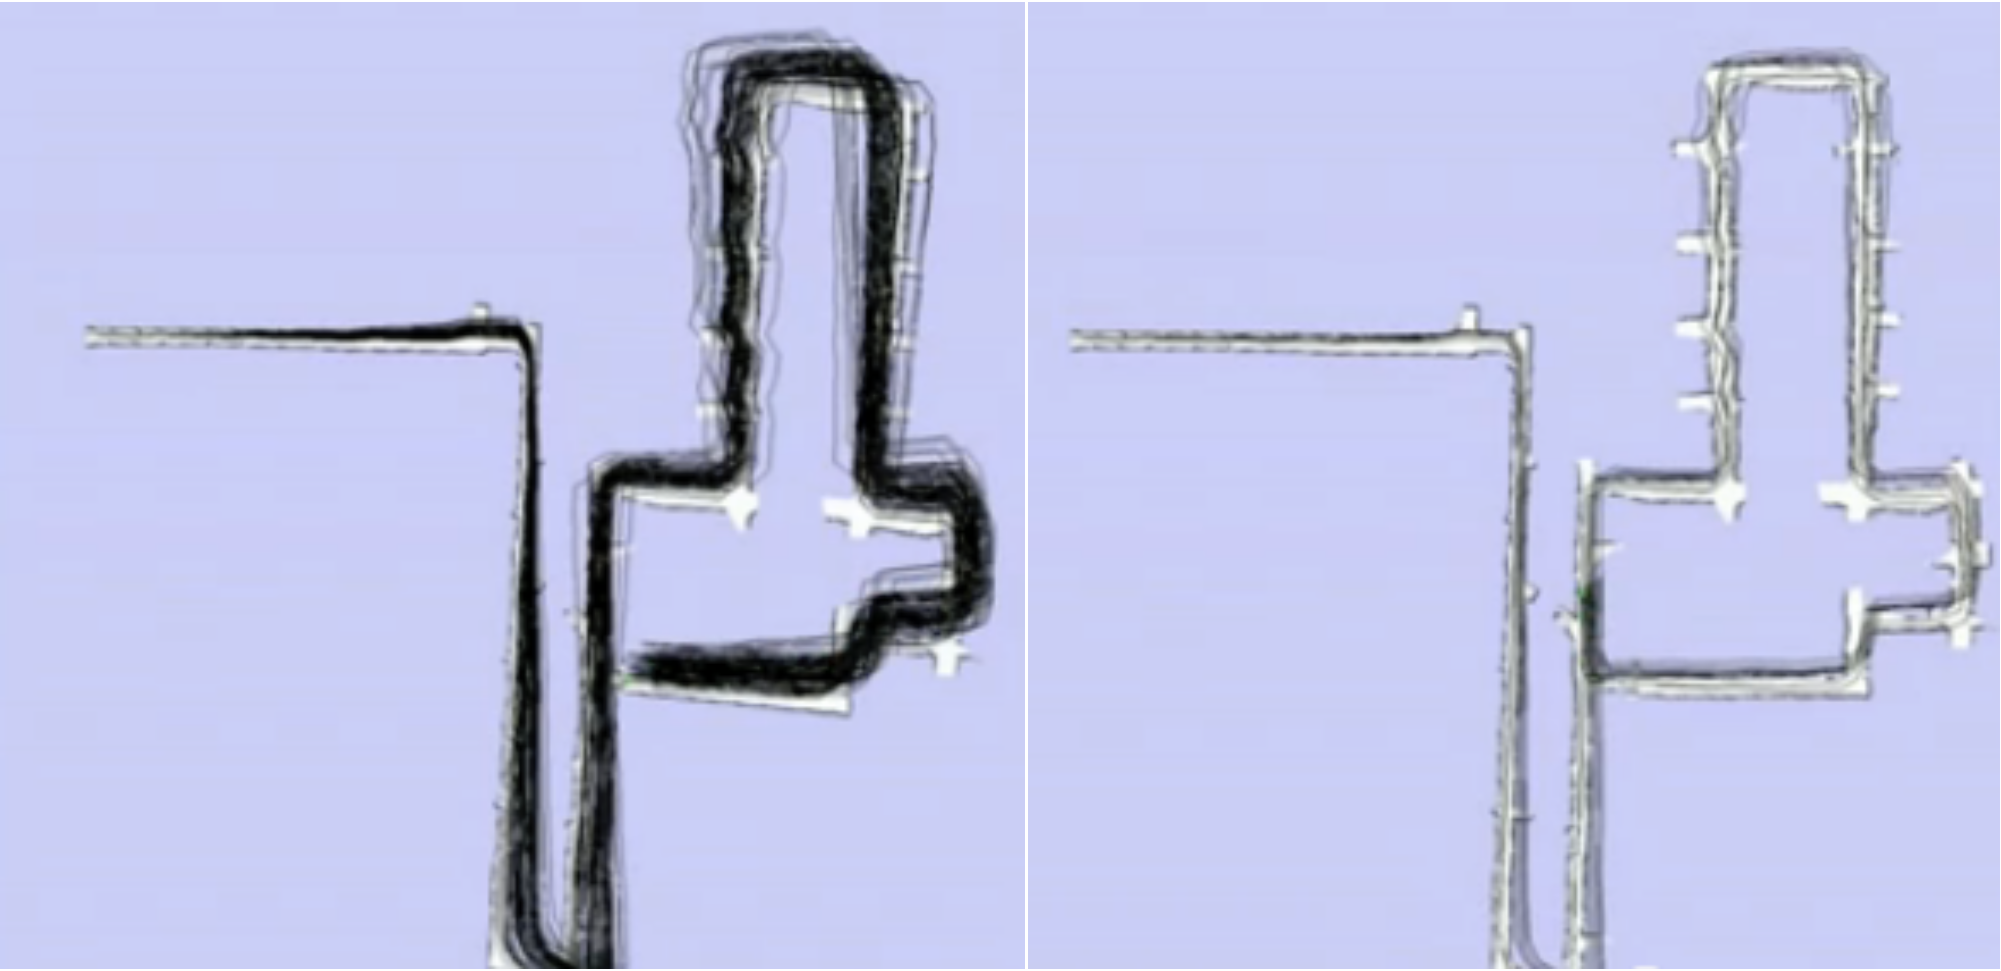
\includegraphics[width=0.9\linewidth]{./Figures/SLAMpath}
	\caption{SLAM in action.}
	\label{fig:slamPath}
\end{figure}\noindent

\end{document}